%%----------------------------------------------------------------------
\section{Computational Roadmaps of Social Simulations and Future}
\label{sec:Computational Roadmaps of Social Simulations}
%% - - - - - - - - - - - - - - - - - - - - - - - - - - - - - - - - - - -

In this project, we also try 
to determine how HPC contributes
to the advancement of research on social simulation or
to clarify the computational power required
for real applications of social simulation.
In this section, we focus on three applications and try
to develop roadmaps for them
\cite{Noda2018a}.

In the development of these roadmaps, 
we adopted two indexes to measure the computational cost,
``number of situations'' and ``complexity of one simulation session''.
We considered exhaustive evaluation by simulation as 
a key methodology of social simulation.
Therefore, to evaluate the model,
examining many conditions and models is important.
The index of ``number of situations'' indicates this number.
Meanwhile,
ordinal computational cost of a simulation,
which is determined by the number of entities and the number
of interactions among the entities,
is important.
In addition, in multiagent simulation,
the computational cost of thinking of each agent is significant.
In the following discussion, we integrate these complexities
as ``complexity of one simulation session''.

%%--------------------------------------------------
\subsection{Evacuation/Pedestrian Simulation}
%% - - - - - - - - - - - - - - - - - - - - - - - - -

The main target of evacuation simulation is not
to find an optimal plan of evacuation for a given disaster situation,
but to evaluate the feasibility and robustness of executable candidates
of evacuation plans or guidance policies.

Several simulations have been performed for 
evaluating such evacuation plans
\cite{Noda2009x}\cite{Noda2010p}\cite{Noda2010y}\cite{Yamashita2014}.
For example, a simulation of an evacuation from
a Tsunami struck city in Tokai area in Japan was performed.
We conducted the following exhaustive simulations considering various sizes and evacuation
policies (evacuee's origin-destination (OD) plans).
The simulation results tell that
the scale of evacuation can be grouped into two categories, namely,
``large'' ($>$ 3,000 evacuees) and
``small'' ($<$ 3,000 evacuees),
and that citizens and local governments should consider at least 
two plans for large- and small-scale evacuations.

We execute the evacuation simulation described above to arrive at
a reference point for illustrating computational costs of various
actual applications.
In the above simulation, we considered the following scenarios:
\begin{itemize}
  \item 2,187 OD plans and
  \item 8 cases of evacuation population (70--10,000 agents).
\end{itemize}
Therefore, in total, 17,497 simulation scenarios were executed
over about 30 days when using a single process on Xeon E5 CPU (2.7 GHz).
We denote this reference point as the rectangle
``city zone, TSUNAMI'' in \figref{fig:Figure-4}.

We can easily extend the simulation scale.
Although a population of only 10,000 is considered in ``city zone, TSUNAMI'',
we can extend the simulation to a more densely populated area such as in Tokyo.
For example,
we performed a similar simulation analysis in the Kanazawa area,
which is located on the coast along the Japan Sea and
experiences snowfall in the winter.
In this case, the population size is similar (about 6,000 agents),
but the number of combinations of scenarios increases to 4,194,304 ($2^{22}$).
The rectangle ``city zone, TSUNAMI and HEAVY SNOW'' in 
\figref{fig:Figure-4} denotes this calculation cost.

We can further extend the simulation to a large scale with a larger number of
scenarios.
Kitasenju area, a large transfer station surrounded by rivers,
has a population of 70,000, and the computational cost of simulating this area is
denoted by ``dense-population zone, complex disaster'' in \figref{fig:Figure-4}.
Because this area is densely populated and complex, 
we have combinations of 44 policy candidates,
that is $2^{44}$ scenarios.
In the case of Tokyo, we need additional computational power.
In \figref{fig:Figure-4}, ``megacity'' corresponds a huge
city such as Tokyo.  In this case, the size of evacuation and the
number of possible scenarios is very large.
Therefore, peta- or exa-scale HPC is required to handle such
simulations.

%%----------------------------------------------------------------------
\begin{figure}
  \centering
  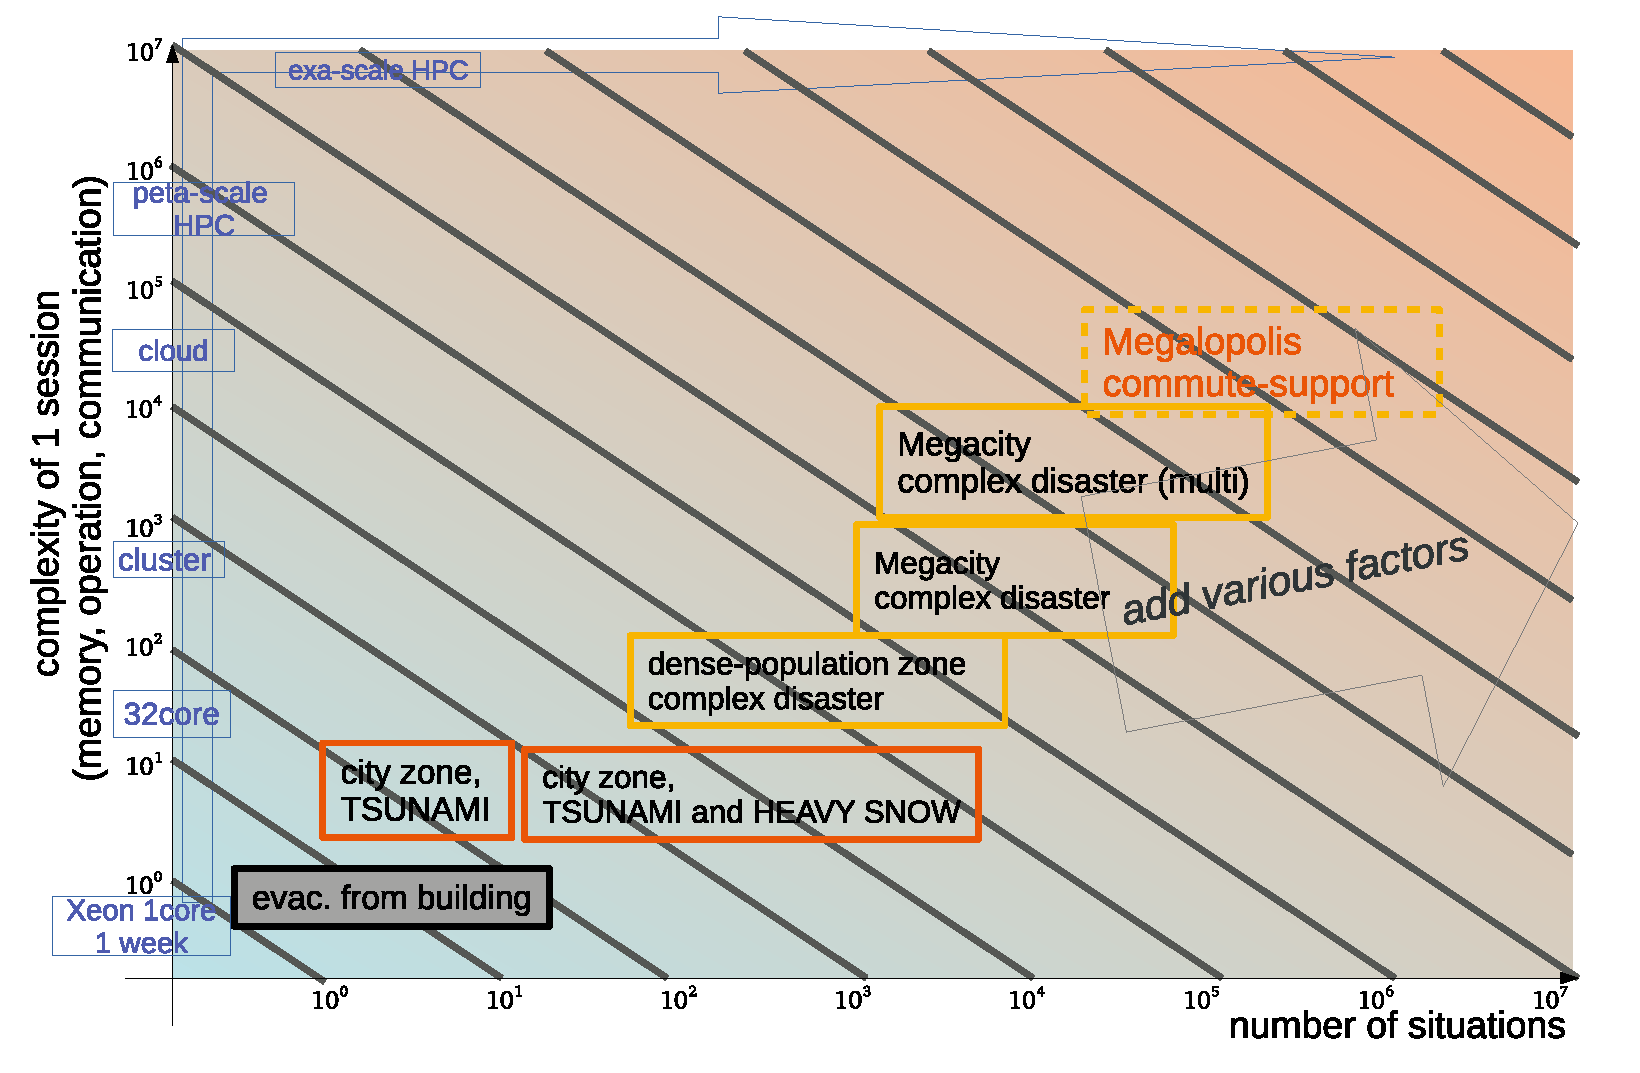
\includegraphics[width=.60\linewidth]{Figs.noda/figure2-4.eps}
  \caption{Roadmap of Evacuation Simulation}
  \label{fig:Figure-4}
\end{figure}
%%----------------------------------------------------------------------

%%--------------------------------------------------
\subsection{Traffic Simulation}
%% - - - - - - - - - - - - - - - - - - - - - - - - -

To create a reference point for the roadmap of the traffic
simulation,
we considered the case of evaluating road restriction policies
for road construction in the Hiroshima area\cite{Osogami2013b}.
In this case, we performed simulations of the following scales:
\begin{itemize}
  \item 70,000 agents (trips), 120,000 road links, and 15 hours and
  \item 20 cases
\end{itemize}
In this case, the calculation required about one day when using a single process
on Xion E5 CPU.
We denote this reference point as ``million city, road plan''
in \figref{fig:Figure-5}.

We can draw out the roadmap from this reference point.
When considering the Tokyo area,
the number of agents increases up to about 2 million
and the number of road links increases to about 610,000.
Moreover, if we consider a larger area such as the Tokyo metropolitan area,
the population increases about 4 million and the number of road links increases to 2.5 million.
These calculation costs are plotted as ``Tokyo, traffic
control'' and ``metropolis, traffic control'' in
\figref{fig:Figure-5}.

When we consider a big event,
we must list a large number of cases to evaluate the robustness
of road traffic to accidents,
whereas the scenarios mentioned above pertain to normal situations
that are repeated every day.
Because various situations affect traffics,
the number of situations increases quickly.
These costs are plotted as 
``Tokyo, big event'', ``metropolis, big event'' and ``whole Japan, big
event''
in \figref{fig:Figure-5}, and they require exa-scale computational power.


%%----------------------------------------------------------------------
\begin{figure}
  \centering
  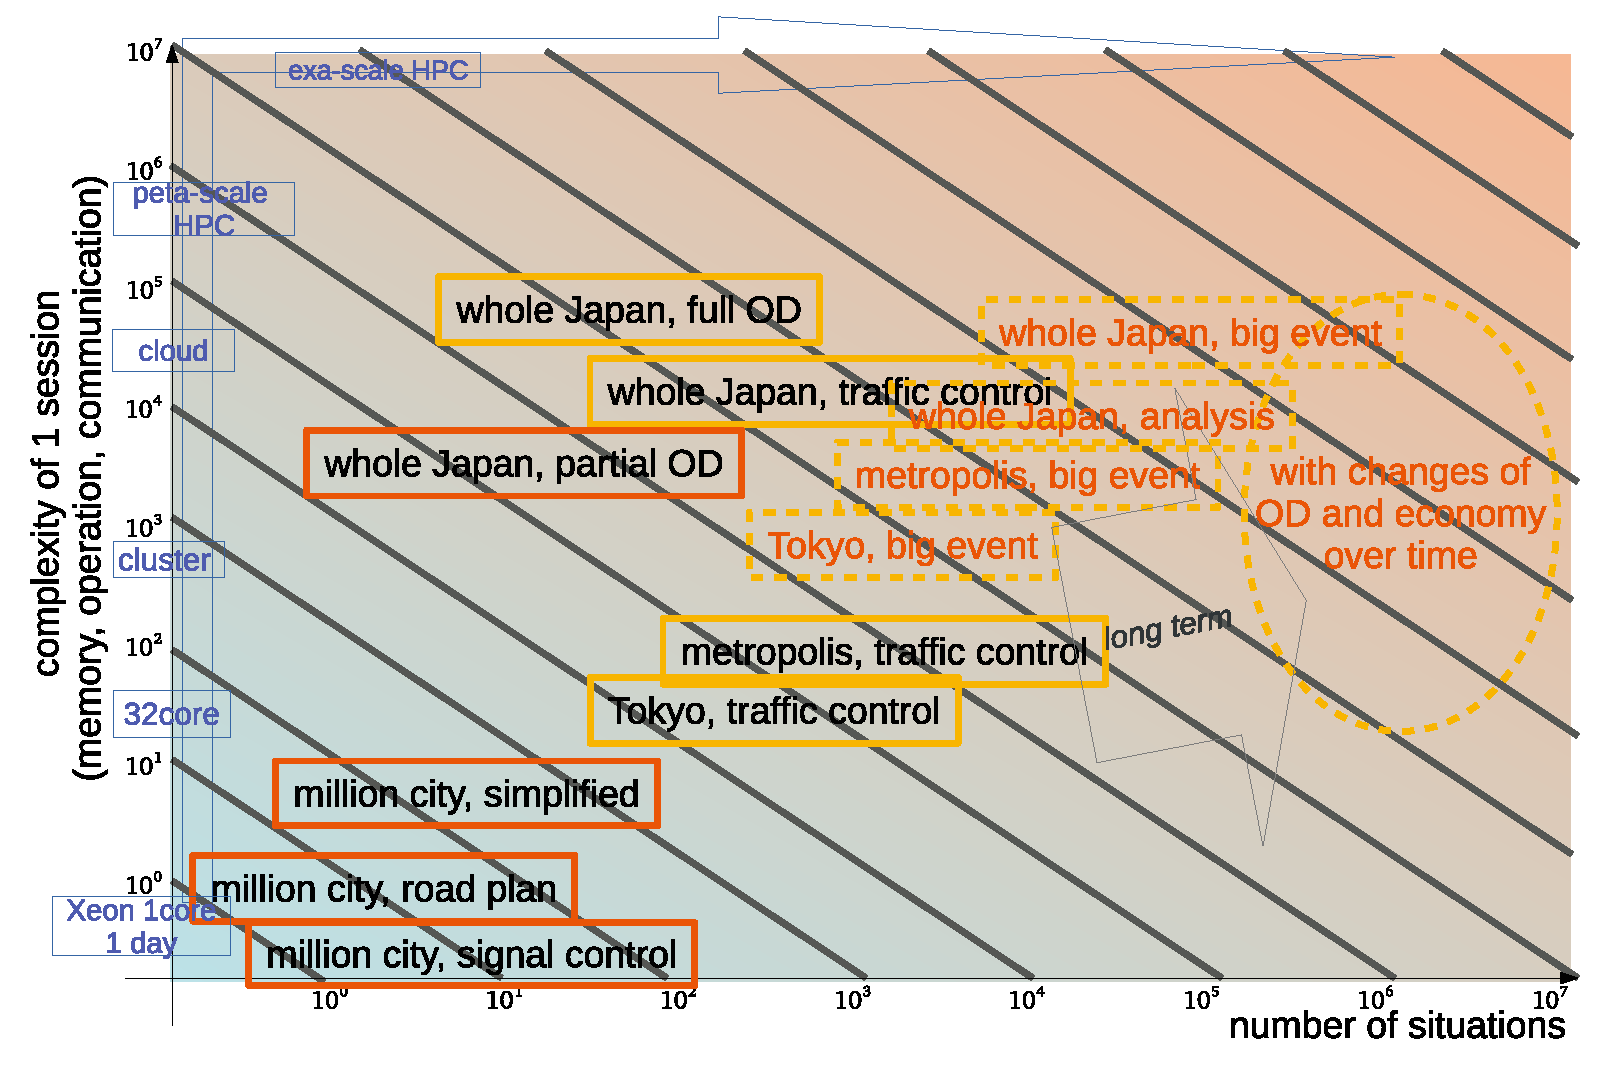
\includegraphics[width=.60\linewidth]{Figs.noda/figure2-5.eps}
  \caption{Roadmap of Traffic Simulation}
  \label{fig:Figure-5}
\end{figure}
%%----------------------------------------------------------------------


%%--------------------------------------------------
\subsection{Market Simulation}
%% - - - - - - - - - - - - - - - - - - - - - - - - -

Market simulations are another important application of multiagent
simulations,
in which agents directly affect each other by selling/buying stocks
and/or currencies \cite{Kawakubo2014a}.
Compared with evacuation and traffic simulations,
market simulations are not constrained by physical space.
Therefore, the time cycles of agents' interactions may be quite short.
Moreover, the ways of thinking of agents show large variations.
This means that the market simulations also require huge
computational cost.

As the reference point of the calculation cost in market simulations,
we present the case of ``tic size'' evaluation.
In this scenario, we conducted a simulation of multiple markets
having different tic sizes,
which is the minimum price unit for trading stocks.
Market companies such as Japan Exchange Group internationally compete
with each other by providing attractive services to traders.
A small tic size
is one of such services that  considerably increases cost.
Therefore, such organizations need evaluations of changes to such services in advance.
In collaborative works with Japan Exchange Group, we conducted a
simulation experiment to find key conditions that determine market share
among markets.
In the simulation, we considered the following scenario:
\begin{itemize}
  \item one good in two markets, 1,000 agents, and 10 million cycles
  \item five cases of tic size and 100 simulation runs per case
\end{itemize}
This simulation takes about one day when using a single thread on a Xeon E5 CPU.
As the reference point, we plot this as ``tic size'' in \figref{fig:Figure-6}.

We are considering extending the market simulations to various
applications used for stock market analyses.
For example, it is in the interest of market companies 
to determine ``daily limit'' and ``cut-off'' prices\cite{Mizuta2013a}.
In this case, the simulation must handle 10--20 goods.
Moreover, evaluating the effects of ``arbitrage'' \cite{Kawakubo2014a}, 
which involves trading rather quickly in intervals of milliseconds,
is important from the viewpoint of maintaining sound market conditions.
This will increase the computational cost, as plotted in \figref{fig:Figure-6}.
Another topic is the evaluation of ``Basel Capital Accords'',
which deal with the soundness of banks in markets.
In the present study, we executed the case of three names for the Basel Accords,
but we will extend it to 100 names in the real application.

The evaluation of ``systemic risks of inter-bank network'' is an important issue
in market evaluation.
However, currently, the 
computational cost of a naive simulation exceeds exa-scale HPC.


%%----------------------------------------------------------------------
\begin{figure}
  \centering
  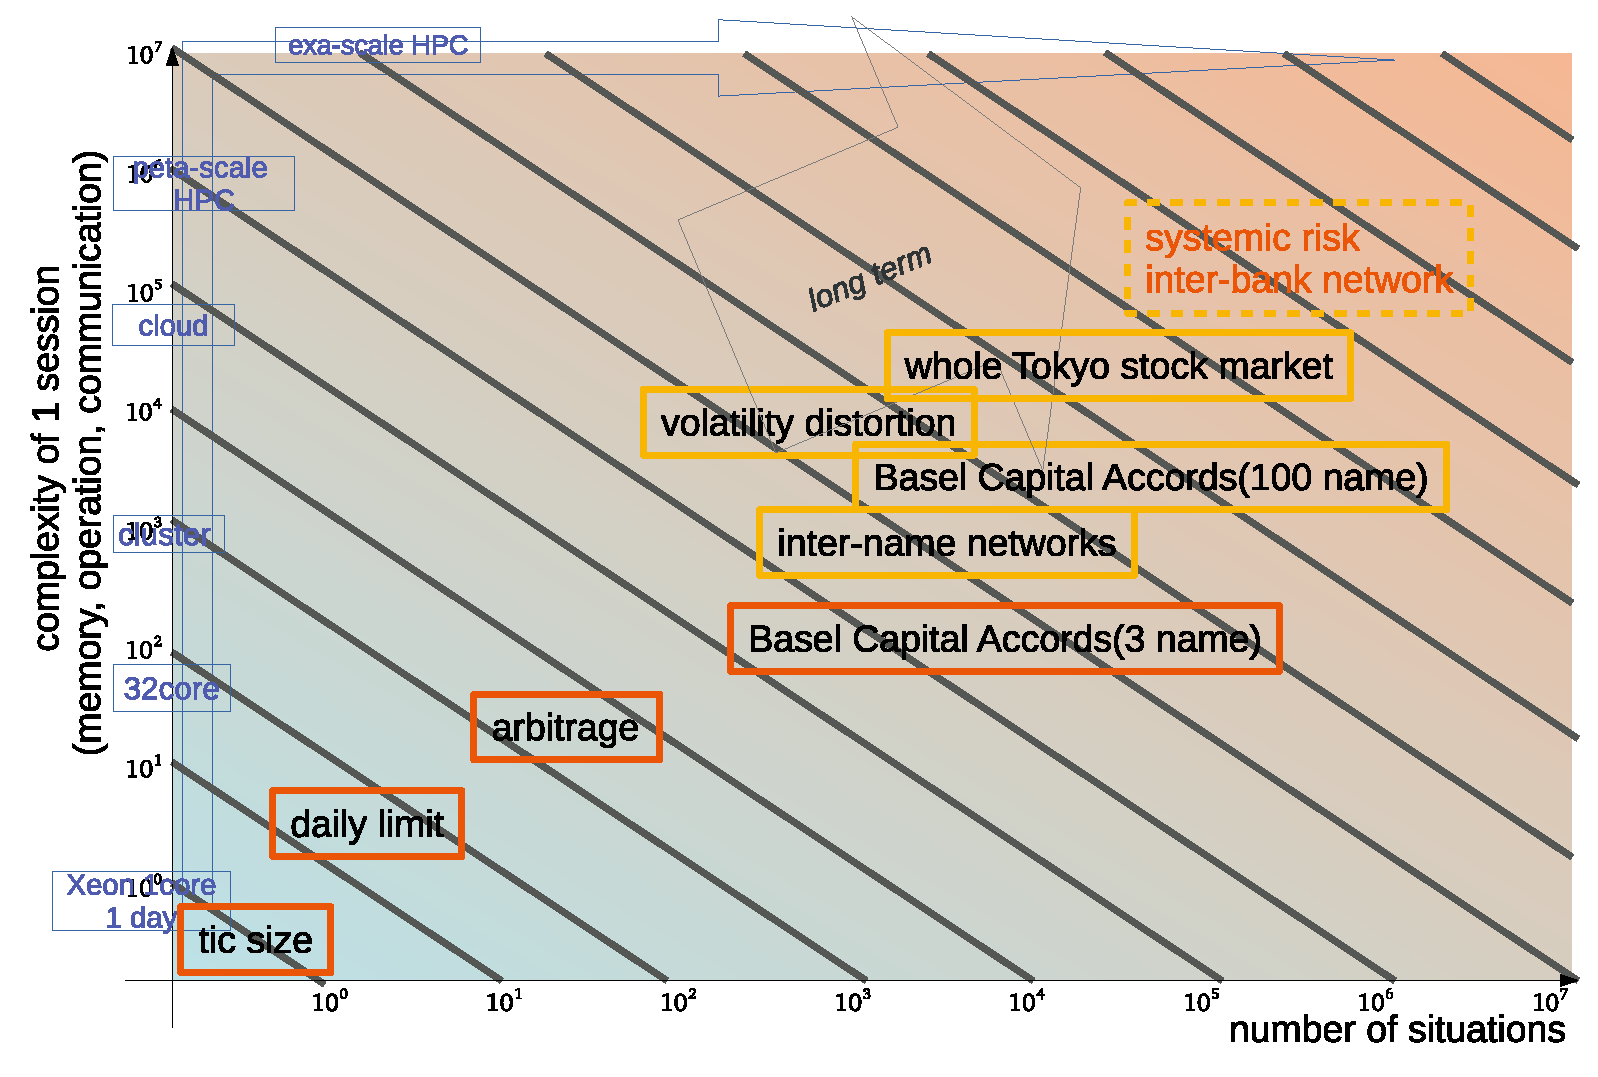
\includegraphics[width=.60\linewidth]{Figs.noda/figure2-6.eps}
  \caption{Roadmap of Market Simulation}
  \label{fig:Figure-6}
\end{figure}
%%----------------------------------------------------------------------

% %%--------------------------------------------------
% \subsection{Transportation Service Simulation}
% %% - - - - - - - - - - - - - - - - - - - - - - - - -
% %%----------------------------------------------------------------------
% \begin{figure}
%   \centering
%   \includegraphics[width=.60\linewidth]{Figs.noda/Figure-8.eps}
%   \caption{Roadmap of Transportation Service Simulation}
%   \label{fig:Figure-8}
% \end{figure}
% %%----------------------------------------------------------------------


%\cite{Noda2013l}

